\documentclass[11pt,a4paper]{article}
\usepackage[utf8]{inputenc}
\usepackage[T1]{fontenc}
\usepackage[norsk]{babel}
\usepackage{tgtermes}
\usepackage{tgheros}
\renewcommand{\ttdefault}{txtt}
\usepackage{amsmath,amssymb}
\usepackage[a4paper,left=2.45cm,right=2.6cm,top=2.3cm,bottom=2.2cm,headsep=0.9cm]{geometry}
\usepackage{fancyhdr}
\usepackage{lastpage}
\usepackage{xcolor}
\usepackage{tikz}
\usepackage{pgfplots}
\pgfplotsset{compat=1.18}
\usepackage{booktabs}
\usepackage{array}
\usepackage{enumitem}
\usepackage{listings}
\usepackage{needspace}
\usepackage{multirow}
\usetikzlibrary{positioning,arrows.meta,calc}
\definecolor{insgrey}{gray}{0.42}
\definecolor{radiogrey}{gray}{0.70}
\setlength{\parindent}{0pt}
\setlength{\parskip}{0.45em}
\setlist[itemize]{itemsep=0pt,topsep=2pt,label=\textbullet,font=\sffamily}
\lstset{basicstyle=\ttfamily\small,columns=fullflexible,keepspaces=true,
  showstringspaces=false,upquote=true,aboveskip=0.6em,belowskip=0.6em,
  literate={æ}{{\ae}}1 {ø}{{\o}}1 {å}{{\aa}}1 {Æ}{{\AE}}1 {Ø}{{\O}}1 {Å}{{\AA}}1}
\pagestyle{fancy}
\fancyhf{}
\renewcommand{\headrulewidth}{0pt}
\fancyhead[R]{\fontsize{7.5}{9}\selectfont\sffamily\color{insgrey}TDT4172 - Introduksjon til maskinlæring - Øvingssett 1}
\fancyfoot[R]{\fontsize{7}{9}\selectfont\sffamily\color{insgrey}\thepage/\pageref{LastPage}}
\newcommand{\delstart}[1]{\clearpage
  \noindent\hspace*{-1.55em}\makebox[1.55em][l]{\sffamily\bfseries\fontsize{12}{14}\selectfont\raisebox{0.35em}{#1}}%
  {\sffamily\bfseries\fontsize{18}{22}\selectfont Part #1}\par\vspace{1.0em}}
\newcommand{\sporsmal}[1]{\par\Needspace{9\baselineskip}\vspace{1.9em}%
  \noindent{\bfseries Spørsmål #1}\par\vspace{-0.45em}%
  \noindent{\bfseries -{}-{}-{}-{}-{}-{}-{}-{}-{}-{}-{}-{}-{}-{}-{}-{}-}\par\vspace{-0.15em}}
\newcommand{\velg}[1]{\par\Needspace{6\baselineskip}\noindent{\bfseries #1}\par\vspace{0.3em}}
\newcommand{\radio}[1]{\tikz[baseline=-0.62ex]{\draw[radiogrey,line width=0.45pt,fill=gray!5] (0,0) circle (0.56em);
  \node[inner sep=0pt,font=\sffamily\fontsize{5.5}{6}\selectfont,text=insgrey] at (0,0) {#1};}}
\newenvironment{alternativer}{\begin{list}{}{\setlength{\leftmargin}{2.35em}\setlength{\labelwidth}{1.4em}%
  \setlength{\labelsep}{0.6em}\setlength{\itemsep}{0.85em}\setlength{\topsep}{0.45em}\setlength{\parsep}{0pt}}%
  \sffamily\fontsize{10}{12.6}\selectfont}{\end{list}}
\newcommand{\alt}[2]{\item[\radio{#1}]#2}
\newcommand{\makspoeng}{\par\vspace{2.2em}\hfill{\sffamily\fontsize{8.5}{10}\selectfont Maks poeng: 10}\hspace*{0.5em}\par}
\begin{document}

\noindent\hspace*{-1.55em}\makebox[1.55em][l]{\raisebox{0.3em}{\sffamily\bfseries\fontsize{11}{12}\selectfont i}}%
{\sffamily\bfseries\fontsize{18}{22}\selectfont Frontpage}\par\vspace{1.1em}

{\bfseries Eksamensoppgave i TDT4172 - Introduksjon til maskinlæring}\\
{\bfseries Øvingssett:} 1 av 10 (uoffisielt øvingssett)\\
{\bfseries Tid:} 4 timer

\vspace{0.6em}
{\bfseries Faglig kontakt:} --- (øvingssett, ikke en offisiell eksamen)\\
{\bfseries Møter i eksamenslokalet:} Nei

\vspace{0.6em}
{\bfseries Hjelpemiddelkode/Tillatte hjelpemidler:} D / Ingen trykte eller håndskrevne hjelpemidler tillatt.
Bestemt, enkel kalkulator tillatt.

\vspace{0.6em}
{\bfseries\underline{ANNEN INFORMASJON:}}

\vspace{0.4em}
{\bfseries Les oppgavene nøye og gjør dine egne antagelser.} Presiser i besvarelsen hvilke forutsetninger du
har lagt til grunn i tolkning/avgrensing av oppgaven.

Dette øvingssettet er laget for egentrening, med samme format og vanskelighetsgrad som de
siste ordinære eksamenene i emnet. Løsningsforslaget står på siste side.

\vspace{1.6em}
{\bfseries\underline{FAGSPESIFIKK INFORMASJON}}

\vspace{0.4em}
{\bfseries Ingen papirhåndtegninger:}\\
Denne eksamenen tillater ikke bruk av håndtegninger.

\vspace{1.4em}
{\bfseries Vekting av oppgavene}:\\
Denne eksamenen inneholder flervalgsoppgaver organisert i ti grupper på fire spørsmål hver. Hver
gruppe vurderes separat etter følgende regler:

\vspace{0.6em}
For hver av de fire spørsmålene i gruppen får du følgende poeng
\begin{itemize}[leftmargin=2.2em,label=\textperiodcentered,itemsep=0pt]
\item {\bfseries Riktig svar:} +2,5 poeng
\item {\bfseries Feil svar (et alternativ er valgt, men ikke korrekt):} $-$0,83 poeng
\item {\bfseries Ikke besvart:} 0 poeng
\end{itemize}
{\bfseries Merk} at dersom du først har valgt et svaralternativ, kan du {\bfseries ikke velge det bort} igjen. Da må du
svare på det spørsmålet. Med andre ord mister du muligheten til å la et spørsmål stå blankt så fort
du har trykket på et alternativ.

\vspace{0.6em}
Poengsummen for hver gruppe er {\bfseries summen} av poengene for de fire enkeltspørsmålene.\\
For {\bfseries alle spørsmålene} gjelder en {\bfseries null-grense}: dersom summen for denne gruppen blir negativ,
settes verdien til {\bfseries 0}. Den totale poengsummen på eksamen er summen av poengene fra alle
gruppene.

\delstart{1}
\sporsmal{1}
Du lager et bar-plott (søylediagram) av Titanic-dataene med \emph{Pclass} på x-aksen og \emph{Survived}
(0/1) som verdi. Søylene for klasse 1, 2 og 3 har høyde 0.63, 0.47 og 0.24.

Hva angir høyden på hver søyle?
\velg{Velg ett alternativ:}
\begin{alternativer}
\alt{A}{Andelen av alle passasjerene som reiste i klassen, altså hvor stor klassen er i datasettet}
\alt{B}{Andelen av alle de overlevende som reiste i klassen, altså fordelingen av Pclass blant overlevende}
\alt{C}{Andelen av passasjerene i klassen som overlevde, altså gjennomsnittet av Survived i klassen}
\alt{D}{Sannsynligheten en trent modell predikerer for overlevelse, gjennomsnittlig over klassen}
\end{alternativer}
\sporsmal{2}
Et datasett med boliger inneholder blant annet følgende features, som alle er lagret som tall:
\begin{itemize}
\item \emph{Postnummer} (f.eks.\ 7030, 7491, 0150)
\item \emph{Antall\_soverom} (0, 1, 2, \ldots)
\item \emph{Byggeår} (f.eks.\ 1962, 2004)
\item \emph{Boligareal} (i m$^2$, med desimaler)
\end{itemize}

Hvilken av disse bør behandles som en \textbf{kvalitativ (kategorisk)} variabel?
\velg{Velg ett alternativ:}
\begin{alternativer}
\alt{A}{Antall soverom, fordi den kun kan ta heltallsverdier og derfor er diskret, ikke kontinuerlig}
\alt{B}{Byggeår, fordi den har et begrenset antall ulike verdier i datasettet}
\alt{C}{Postnummer, fordi tallene bare er koder, og differansen mellom to koder har ingen mening}
\alt{D}{Boligareal, fordi kontinuerlige verdier må deles inn i intervaller før de kan brukes}
\end{alternativer}
\sporsmal{3}
Featuren \emph{Region} har fem verdier (Nord, Midt, Vest, Øst, Sør) uten noen naturlig rekkefølge. Du koder
den med \texttt{LabelEncoder} til tallene 0--4 og bruker den som én input-feature i en logistisk
regresjonsmodell.

Hvilket utsagn om denne kodingen er riktig?
\velg{Velg ett alternativ:}
\begin{alternativer}
\alt{A}{Modellen får bare én vekt for Region og tolker dermed avstanden mellom kodene som meningsfull}
\alt{B}{Kodingen gjør tapsfunksjonen ikke-konveks, siden Region bare kan ta et fåtall heltallsverdier}
\alt{C}{Kodingen er tilstrekkelig, siden logistisk regresjon bare krever at alle features er numeriske}
\alt{D}{Kodingen er uproblematisk så lenge kodene 0--4 skaleres til $[0,1]$ med \texttt{MinMaxScaler} først}
\end{alternativer}
\sporsmal{4}
Et datasett har features $x_1$ og $x_2$, som begge kan være positive eller negative. Klasse 1 består av
punktene der $x_1$ og $x_2$ har \textbf{samme fortegn}, og klasse 0 av punktene der de har ulikt fortegn.
En logistisk regresjonsmodell trent på $(x_1, x_2)$ får en accuracy rundt 50\,\%.

Hvilken ekstra feature gjør det mulig for logistisk regresjon å skille klassene godt?
\velg{Velg ett alternativ:}
\begin{alternativer}
\alt{A}{$x_1 + x_2$, siden klassen er bestemt av fortegnet til summen}
\alt{B}{$|x_1|$, siden klassen er bestemt av avstanden fra $x_2$-aksen}
\alt{C}{$x_1^2 + x_2^2$, siden klassen er bestemt av avstanden fra origo}
\alt{D}{$x_1 x_2$, siden klassen er bestemt av fortegnet til produktet}
\end{alternativer}
\makspoeng

\delstart{2}
\sporsmal{1}
En binær klassifiseringsmodell gir følgende \textbf{confusion matrix} på testdata:
\begin{center}
\begin{tabular}{lcc}
\toprule
 & Predikert positiv & Predikert negativ\\
\midrule
Faktisk positiv & 40 & 10\\
Faktisk negativ & 20 & 130\\
\bottomrule
\end{tabular}
\end{center}
Hva er modellens \textbf{precision} og \textbf{recall}?
\velg{Velg ett alternativ:}
\begin{alternativer}
\alt{A}{Precision $= 0.80$ og recall $= 0.67$}
\alt{B}{Precision $= 0.67$ og recall $= 0.80$}
\alt{C}{Precision $= 0.85$ og recall $= 0.87$}
\alt{D}{Precision $= 0.33$ og recall $= 0.20$}
\end{alternativer}
\sporsmal{2}
Et spamfilter testes på 1000 e-poster, hvorav 100 er spam (positiv klasse). Filteret flagger
95 e-poster som spam, og 80 av disse er faktisk spam.

Hva er filterets \textbf{spesifisitet} (TNR) og \textbf{false positive rate} (FPR)?
\velg{Velg ett alternativ:}
\begin{alternativer}
\alt{A}{TNR $= 0.983$ og FPR $= 0.017$}
\alt{B}{TNR $= 0.800$ og FPR $= 0.200$}
\alt{C}{TNR $= 0.842$ og FPR $= 0.158$}
\alt{D}{TNR $= 0.978$ og FPR $= 0.022$}
\end{alternativer}
\sporsmal{3}
Et treningssett har 95\,\% datapunkter med label $y=0$ og 5\,\% med $y=1$. Du bruker den vektede tapsfunksjonen
\[ L(y_{pred}, y) = -w_1\, y \ln y_{pred} - w_0\,(1-y)\ln(1-y_{pred}) \]
og ønsker at de to klassene skal bidra omtrent like mye til det totale tapet.

Hvilket valg av vekter oppnår dette?
\velg{Velg ett alternativ:}
\begin{alternativer}
\alt{A}{$w_0 = 0.95$ og $w_1 = 0.05$, slik at vektene speiler klassefordelingen i dataene}
\alt{B}{$w_0 = 0.5$ og $w_1 = 0.5$, slik at begge klassene vektes likt i tapsfunksjonen}
\alt{C}{$w_0 = 19$ og $w_1 = 1$, slik at klassen med flest eksempler straffes hardest}
\alt{D}{$w_0 = 1$ og $w_1 = 19$, slik at feil på klasse 1 straffes 19 ganger så hardt}
\end{alternativer}
\sporsmal{4}
Du har 1000 datapunkter, hvorav 2\,\% tilhører den positive klassen, og skal dele dataene i 80\,\% trening og
20\,\% test. En kollega foreslår å bruke \textbf{stratifisert splitting} i stedet for en helt tilfeldig splitt.

Hva oppnår stratifisert splitting her?
\velg{Velg ett alternativ:}
\begin{alternativer}
\alt{A}{Begge settene får samme klassefordeling som hele datasettet, altså 2\,\% positive}
\alt{B}{Splitten blir deterministisk, slik at de samme punktene havner i testsettet hver gang}
\alt{C}{Trenings- og testsettet får like mange positive som negative eksempler}
\alt{D}{Den positive klassen oversamples i treningssettet, slik at modellen ser flere positive}
\end{alternativer}
\makspoeng

\delstart{3}
\sporsmal{1}
Et beslutningstre bruker \textbf{entropi} som splittkriterium og velger i hver node splitten med størst
informasjonsgevinst $\Delta I = I_{\text{før}} - E[I_{\text{etter}}]$. En kollega bytter fra $\log_2$ til
naturlig logaritme $\ln$ i entropiformelen $I = -\sum_i p_i \log p_i$ og trener på nytt med de samme dataene.

Hva skjer med treet?
\velg{Velg ett alternativ:}
\begin{alternativer}
\alt{A}{Entropien kan bli negativ for nesten rene noder, så enkelte splitter kan få negativ gevinst}
\alt{B}{Maksimal entropi for to klasser er fortsatt 1, men gevinstene bytter rekkefølge for noder med skjev fordeling}
\alt{C}{Alle entropier og gevinster ganges med samme faktor $\ln 2$, så treet velger nøyaktig de samme splittene}
\alt{D}{Entropien blir høyere for urene noder, så treet foretrekker splitter som gir helt rene barnenoder}
\end{alternativer}
\sporsmal{2}
En Naive Bayes-klassifikator er trent på 900 punkter fra klasse 0 og 100 fra klasse 1. Du oversampler
klasse 1 slik at hvert av de 100 punktene forekommer nøyaktig ni ganger (originalen pluss åtte kopier).
Begge klassene har da 900 punkter, og du trener på nytt.

Hvilke ledd i $p(C_k)\prod_i p(x_i \mid C_k)$ får nye verdier?
\velg{Velg ett alternativ:}
\begin{alternativer}
\alt{A}{Både prioren og likelihoodene, siden alle sannsynlighetene estimeres på nytt fra de nye dataene}
\alt{B}{Bare likelihoodene $p(x_i \mid C_1)$, som nå estimeres fra ni ganger så mange punkter}
\alt{C}{Bare prioren $p(C_k)$, som går fra 0.1 til 0.5 for klasse 1; likelihoodene er uendret}
\alt{D}{Ingen av leddene, siden kopier ikke tilfører noen ny informasjon om klassene}
\end{alternativer}
\sporsmal{3}
Et datasett har features $x_1, x_2 \in [0, 10]$, og klassen er 1 hvis $x_2 > x_1$ og 0 ellers. Du trener et
beslutningstre (\texttt{DecisionTreeClassifier}) på mange slike punkter, med originale features.

Hvordan ser beslutningsgrensen til treet ut?
\velg{Velg ett alternativ:}
\begin{alternativer}
\alt{A}{En rett diagonal linje allerede etter én splitt, siden treet kan splitte direkte på $x_2 - x_1$}
\alt{B}{Ingen nyttig grense, siden et tre bare kan skille klasser som er separerbare langs én enkelt akse}
\alt{C}{En glatt kurve rundt diagonalen, siden Gini-urenheten minimeres kontinuerlig under treningen}
\alt{D}{En trapp av kun vertikale og horisontale segmenter rundt diagonalen, finere jo dypere treet er}
\end{alternativer}
\sporsmal{4}
En node i et beslutningstre har 30\,\% av punktene i klasse 1 og 70\,\% i klasse 0, og Gini-urenheten
er $1 - 0.3^2 - 0.7^2 = 0.42$.

Hvilken tolkning av tallet 0.42 er riktig?
\velg{Velg ett alternativ:}
\begin{alternativer}
\alt{A}{Andelen av punktene i noden som blir feilklassifisert når noden predikerer majoritetsklassen}
\alt{B}{Sannsynligheten for at to tilfeldig trukne punkter fra noden tilhører samme klasse}
\alt{C}{Hvor mye entropien i noden vil reduseres hvis noden splittes videre på den beste featuren}
\alt{D}{Sannsynligheten for feil når et tilfeldig punkt i noden får et label trukket etter nodens klassefordeling}
\end{alternativer}
\makspoeng

\delstart{4}
\sporsmal{1}
En lineær regresjonsmodell $f(x) = 2x + 1$ evalueres på fire datapunkter:
\begin{center}
\begin{tabular}{ccccc}
\toprule
$x$ & 0 & 1 & 2 & 3\\
\midrule
$y$ & 1.5 & 2 & 6 & 6\\
\bottomrule
\end{tabular}
\end{center}
Hva blir $\text{MSE} = \frac{1}{N}\sum_{i=1}^{N}\big(y^{(i)} - f(x^{(i)})\big)^2$ (uten faktoren $\tfrac12$)?
\velg{Velg ett alternativ:}
\begin{alternativer}
\alt{A}{$0.88$}
\alt{B}{$0.81$}
\alt{C}{$1.63$}
\alt{D}{$3.25$}
\end{alternativer}
\sporsmal{2}
En lineær regresjonsmodell $f(x) = \beta_0 + \beta_1 x$ trenes med gradient descent på MSE, med
\[ \frac{\partial L}{\partial \beta_0} = \frac{1}{N}\sum_{i=1}^{N}\big(f(x^{(i)}) - y^{(i)}\big),
\qquad \beta_0 \leftarrow \beta_0 - \eta\,\frac{\partial L}{\partial \beta_0}. \]
Den nåværende modellen \textbf{overestimerer} target for alle treningspunktene.

Hva gjelder for neste oppdatering av $\beta_0$?
\velg{Velg ett alternativ:}
\begin{alternativer}
\alt{A}{$\partial L/\partial\beta_0 < 0$, og oppdateringen gjør $\beta_0$ mindre}
\alt{B}{$\partial L/\partial\beta_0 > 0$, og oppdateringen gjør $\beta_0$ mindre}
\alt{C}{$\partial L/\partial\beta_0 > 0$, og oppdateringen gjør $\beta_0$ større}
\alt{D}{$\partial L/\partial\beta_0 < 0$, og oppdateringen gjør $\beta_0$ større}
\end{alternativer}
\sporsmal{3}
Du trener en modell med \textbf{early stopping} og tålmodighet (patience) på 5 epoker.

Hvilken beskrivelse av early stopping er riktig?
\velg{Velg ett alternativ:}
\begin{alternativer}
\alt{A}{Treningen stanses når testtapet ikke har blitt bedre de siste 5 epokene}
\alt{B}{Treningen stanses når treningstapet ikke har blitt bedre de siste 5 epokene}
\alt{C}{Treningen stanses alltid etter 5 epoker, slik at modellen ikke rekker å overtilpasse}
\alt{D}{Treningen stanses når valideringstapet ikke har blitt bedre de siste 5 epokene}
\end{alternativer}
\sporsmal{4}
Et \textbf{regresjonstre} skal predikere boligpriser.

Hva predikerer treet for et nytt punkt, og hvordan velges splittene?
\velg{Velg ett alternativ:}
\begin{alternativer}
\alt{A}{Gjennomsnittet av target i løvnoden; splittene velges for å minimere Gini-urenheten}
\alt{B}{Medianen av target i løvnoden; splittene velges for å minimere Gini-urenheten}
\alt{C}{Gjennomsnittet av target i løvnoden; splittene velges for å minimere MSE i barnenodene}
\alt{D}{Medianen av target i løvnoden; splittene velges for å minimere MSE i barnenodene}
\end{alternativer}
\makspoeng

\delstart{5}
\sporsmal{1}
Et parallelt ensemble av fem klassifiseringstrær skal bestemme arten til en pingvin i Palmer Penguins-dataene.
Artene er kodet som Adelie $=0$, Chinstrap $=1$ og Gentoo $=2$. For én pingvin predikerer de fem trærne
\[ 0,\quad 0,\quad 0,\quad 2,\quad 2 . \]
En kollega aggregerer med \texttt{np.round(np.mean(preds))} i stedet for flertallsavstemning.

Hvilket utsagn om kollegaens aggregering er riktig?
\velg{Velg ett alternativ:}
\begin{alternativer}
\alt{A}{Den gir Adelie, fordi snittet av kodene alltid havner nærmest arten som flest av trærne har stemt på}
\alt{B}{Den gir Chinstrap, en art ingen av trærne stemte på, fordi kodene 0--2 ikke har noen meningsfull rekkefølge}
\alt{C}{Den gir Chinstrap, og det er rimelig, siden snittet tar hensyn til at to av trærne stemte på Gentoo}
\alt{D}{Den gir samme resultat som flertallsavstemning, men regnes som vektet avstemning der trærne teller likt}
\end{alternativer}
\sporsmal{2}
Fra tre datapunkter $\{a,\ b,\ c\}$ trekker du ett bootstrap-utvalg av størrelse 3, altså tre trekk med
tilbakelegging.

Hva er sannsynligheten for at utvalget inneholder alle tre punktene (ingen duplikater)?
\velg{Velg ett alternativ:}
\begin{alternativer}
\alt{A}{$0.70$}
\alt{B}{$0.22$}
\alt{C}{$0.30$}
\alt{D}{$0.67$}
\end{alternativer}
\sporsmal{3}
Du trener gradient boosting for regresjon og halverer læringsraten (shrinkage) fra 0.2 til 0.1, men lar
alt annet være som før.

Hva er den mest sannsynlige effekten?
\velg{Velg ett alternativ:}
\begin{alternativer}
\alt{A}{Hvert tre bidrar mindre, så det trengs flere trær for å nå samme treningsfeil}
\alt{B}{Hvert tre trenes på halvparten av dataene, så treningen går raskere, men blir mer støyete}
\alt{C}{Pseudo-residualene halveres, så ensemblet undertilpasser uansett hvor mange trær som brukes}
\alt{D}{Hvert tre bidrar mindre, så det trengs færre trær, siden ensemblet overskyter mindre}
\end{alternativer}
\sporsmal{4}
Du trener ti nevrale nettverk med samme arkitektur på de samme treningsdataene, men med ulike tilfeldige
startverdier (random seeds), og bruker gjennomsnittet av de ti prediksjonene.

Hvilket utsagn om dette ensemblet er riktig?
\velg{Velg ett alternativ:}
\begin{alternativer}
\alt{A}{Det er et sekvensielt ensemble, siden hvert nettverk starter fra vektene til det forrige og retter feilene}
\alt{B}{Det kan gi en viss gevinst, men bare hvis nettverkene i tillegg trenes på ulike features eller ulike data}
\alt{C}{Det er et parallelt ensemble, siden nettverkene trenes uavhengig og ender med ulike vekter og feil}
\alt{D}{Det er bagging, siden ulike startverdier gjør at hvert nettverk i praksis lærer av et eget utvalg av dataene}
\end{alternativer}
\makspoeng

\delstart{6}
\sporsmal{1}
Et perceptron har vekter $\mathbf{w} = (0.5,\,-1.0,\,2.0)$, bias $b = -0.5$ og aktiveringsfunksjonen
\[ H(z) = \begin{cases} 1 & \text{hvis } z \geq 0\\ 0 & \text{ellers} \end{cases}, \qquad z = \mathbf{w}^T\mathbf{x} + b. \]
Hva blir $z$ og output for input $\mathbf{x} = (2,\,1,\,0.25)$?
\velg{Velg ett alternativ:}
\begin{alternativer}
\alt{A}{$z = 0.0$ og output $0$}
\alt{B}{$z = 0.0$ og output $1$}
\alt{C}{$z = 0.5$ og output $1$}
\alt{D}{$z = -0.5$ og output $0$}
\end{alternativer}
\sporsmal{2}
Et perceptron med to inputs har $w_1 = 0.2$, $w_2 = -0.4$ og bias $b = 0.1$, og bruker
$\hat y = 1$ hvis $w_1x_1 + w_2x_2 + b \geq 0$, ellers $\hat y = 0$. Læringsregelen er
\[ w_i \leftarrow w_i + \eta\,(y - \hat y)\,x_i, \qquad b \leftarrow b + \eta\,(y - \hat y), \]
med $\eta = 0.5$. Perceptronet får treningspunktet $\mathbf{x} = (1,\,2)$ med $y = 1$.

Hva blir parametrene etter én oppdatering?
\velg{Velg ett alternativ:}
\begin{alternativer}
\alt{A}{$w_1 = -0.3$, $w_2 = -1.4$ og $b = -0.4$}
\alt{B}{$w_1 = 0.7$, $w_2 = 0.1$ og $b = 0.6$}
\alt{C}{$w_1 = 0.2$, $w_2 = -0.4$ og $b = 0.1$}
\alt{D}{$w_1 = 0.7$, $w_2 = 0.6$ og $b = 0.6$}
\end{alternativer}
\sporsmal{3}
Et dypt nevralt nettverk med \textbf{sigmoid} som aktiveringsfunksjon i alle ti skjulte lag trenes med
backpropagation. Vektene i de første lagene endrer seg nesten ikke, mens de siste lagene lærer normalt.

Hva er den mest sannsynlige forklaringen?
\velg{Velg ett alternativ:}
\begin{alternativer}
\alt{A}{Sigmoid gir output i $(0,1)$, så aktiveringene i de første lagene blir for små til å oppdateres}
\alt{B}{Den deriverte $\sigma(z)(1-\sigma(z))$ er størst når $|z|$ er stor, så gradienten eksploderer bakover}
\alt{C}{Den deriverte $\sigma(z)(1-\sigma(z))$ er aldri over 0.25, så gradienten krymper for hvert lag bakover}
\alt{D}{Sigmoid er ikke deriverbar i $z = 0$, så gradienten blir udefinert for noder i de første lagene}
\end{alternativer}
\sporsmal{4}
Du bygger en modell i Keras slik:
\begin{lstlisting}[language=Python]
model = Sequential()
model.add(Dense(8, activation="relu"))
model.add(Dense(1, activation="sigmoid"))
print(model.weights)
\end{lstlisting}
Hva skriver den siste linjen ut?
\velg{Velg ett alternativ:}
\begin{alternativer}
\alt{A}{Tilfeldig initialiserte vekter, fordi \texttt{Dense} oppretter vektene når laget legges til}
\alt{B}{En tom liste, fordi modellen ikke kjenner input-dimensjonen og ikke har opprettet vektene}
\alt{C}{Vekter som er null, fordi modellen ennå ikke er trent med \texttt{model.fit}}
\alt{D}{En feilmelding, fordi modellen må kompileres med \texttt{model.compile} før vektene finnes}
\end{alternativer}
\makspoeng

\delstart{7}
\sporsmal{1}
k-means med $k = 2$ har konvergert på de endimensjonale punktene $1,\ 2,\ 6,\ 9,\ 13$, med klyngene
$\{1, 2, 6\}$ og $\{9, 13\}$.

Hva er inertia for denne løsningen?
\velg{Velg ett alternativ:}
\begin{alternativer}
\alt{A}{$10.0$}
\alt{B}{$22.0$}
\alt{C}{$15.0$}
\alt{D}{$4.4$}
\end{alternativer}
\sporsmal{2}
I oppdateringssteget i \textbf{k-means} flyttes hver sentroide til gjennomsnittet av punktene som er
tilordnet klyngen.

Hvorfor er nettopp gjennomsnittet det riktige valget, gitt hva k-means minimerer?
\velg{Velg ett alternativ:}
\begin{alternativer}
\alt{A}{Gjennomsnittet er alltid punktet som minimerer summen av kvadrerte avstander innad i klyngen}
\alt{B}{Gjennomsnittet er punktet som minimerer summen av absolutte avstander til punktene i klyngen}
\alt{C}{Gjennomsnittet er punktet som maksimerer avstanden til sentroidene i de andre klyngene}
\alt{D}{Gjennomsnittet er alltid et av datapunktene, slik at sentroiden havner i et tett område}
\end{alternativer}
\sporsmal{3}
DBSCAN brukes på punktene under, med $\varepsilon = 1.5$ og \texttt{min\_samples} $= 4$. Et punkt er et
kjernepunkt hvis minst 4 punkter (punktet selv medregnet) ligger innenfor avstand $\leq \varepsilon$.
Punktet $M$ ligger i $x = 3.5$.
\begin{center}
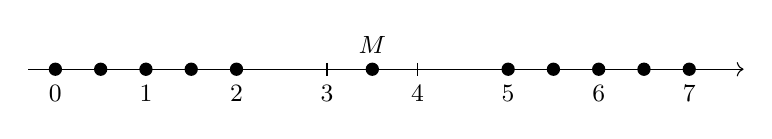
\begin{tikzpicture}[x=1.15cm]
\draw[->] (-0.3,0) -- (7.6,0);
\foreach \t in {0,...,7} \draw (\t,0.08) -- (\t,-0.08) node[below,font=\small] {\t};
\foreach \p in {0,0.5,1,1.5,2,5,5.5,6,6.5,7} \fill (\p,0) circle (2.4pt);
\fill (3.5,0) circle (2.4pt) node[above=2pt,font=\small] {$M$};
\end{tikzpicture}
\end{center}
Hva blir resultatet?
\velg{Velg ett alternativ:}
\begin{alternativer}
\alt{A}{To klynger; $M$ blir kantpunkt i én av dem, men slår ikke klyngene sammen}
\alt{B}{Én klynge; $M$ ligger innenfor $\varepsilon$ av kjernepunkter på begge sider og binder dem sammen}
\alt{C}{To klynger; $M$ blir støy, siden den har færre enn 4 punkter innenfor $\varepsilon$}
\alt{D}{Tre klynger; $M$ danner sin egen lille klynge mellom de to gruppene}
\end{alternativer}
\sporsmal{4}
Du bruker DBSCAN på et datasett med tre tydelige, godt separerte klynger, men velger en
\textbf{altfor stor} verdi for $\varepsilon$ (og en fornuftig \texttt{min\_samples}).

Hva er det mest sannsynlige resultatet?
\velg{Velg ett alternativ:}
\begin{alternativer}
\alt{A}{Antall klynger øker, fordi hvert tett område deles opp i flere mindre klynger}
\alt{B}{Svært mange punkter får nok naboer til å bli kjernepunkter, og gruppene slås sammen til én}
\alt{C}{Nesten alle punkter blir støy, fordi få punkter har nok naboer innenfor $\varepsilon$}
\alt{D}{Klyngene blir de samme, men flere punkter blir kantpunkter i stedet for kjernepunkter}
\end{alternativer}
\makspoeng

\delstart{8}
\sporsmal{1}
I PCA finner vi egenverdier og egenvektorer for dataenes kovariansmatrise.

Hvilket utsagn er riktig?
\velg{Velg ett alternativ:}
\begin{alternativer}
\alt{A}{Hovedkomponentene er de opprinnelige featurene sortert etter varians, og egenverdiene er disse variansene}
\alt{B}{Hovedkomponentene er egenvektorene, og hver egenverdi er antallet opprinnelige features i sin komponent}
\alt{C}{Hovedkomponentene er kolonnene i kovariansmatrisen, og egenverdiene er korrelasjonene mellom features}
\alt{D}{Hovedkomponentene er egenvektorene, og hver egenverdi er variansen til dataene langs sin komponent}
\end{alternativer}
\sporsmal{2}
PCA på et datasett med fire features gir egenverdiene
\[ \lambda_1 = 4.2,\quad \lambda_2 = 2.1,\quad \lambda_3 = 1.2,\quad \lambda_4 = 0.5. \]
Hvor stor andel av den totale variansen bevares om vi beholder de to første hovedkomponentene?
\velg{Velg ett alternativ:}
\begin{alternativer}
\alt{A}{$50\,\%$}
\alt{B}{$66\,\%$}
\alt{C}{$79\,\%$}
\alt{D}{$53\,\%$}
\end{alternativer}
\sporsmal{3}
Du har tilpasset PCA med \texttt{pca.fit(X\_train)} og kjører deretter \texttt{pca.transform(X\_test)}.

Hva gjør det siste kallet?
\velg{Velg ett alternativ:}
\begin{alternativer}
\alt{A}{Sentrerer med gjennomsnittet fra treningsdata og projiserer på hovedkomponentene som ble funnet der}
\alt{B}{Beregner nye hovedkomponenter fra testdataene og projiserer testpunktene på disse komponentene}
\alt{C}{Velger ut de opprinnelige featurene i testdataene som hadde høyest varians i treningsdataene}
\alt{D}{Projiserer testpunktene på komponentene fra treningsdata, men trekker fra testsettets eget gjennomsnitt}
\end{alternativer}
\sporsmal{4}
SNE og t-SNE flytter punktene i embeddingen slik at KL-divergensen
\[ D_{KL}(P\,\|\,Q) = \sum_x P(x)\ln\frac{P(x)}{Q(x)} \]
blir minst mulig. For ett punkt $\mathbf{x}_i$ med to naboer er naboskapsfordelingen i originalrommet
$P = (0.5,\ 0.5)$, mens den i embeddingen er $Q = (0.8,\ 0.2)$.

Hva er $D_{KL}(P\,\|\,Q)$?
\velg{Velg ett alternativ:}
\begin{alternativer}
\alt{A}{$0.22$}
\alt{B}{$0.45$}
\alt{C}{$0.32$}
\alt{D}{$0.19$}
\end{alternativer}
\makspoeng

\delstart{9}
\sporsmal{1}
En agent trenes i Frozen Lake (\texttt{is\_slippery=False}), der reward er 1 når målet nås og ellers 0.
Etter én handling returnerer
\begin{lstlisting}[language=Python]
next_state, reward, done, truncated, info = env.step(action)
\end{lstlisting}
verdiene \texttt{reward = 0}, \texttt{done = True} og \texttt{truncated = False}.

Hva har skjedd?
\velg{Velg ett alternativ:}
\begin{alternativer}
\alt{A}{Agenten nådde målet, siden \texttt{done = True} betyr at oppgaven er løst}
\alt{B}{Agenten falt i et hull, siden episoden er over uten at målet er nådd}
\alt{C}{Agenten nådde målet, men rewarden for målet gis først i neste kall til \texttt{env.step}}
\alt{D}{Agenten gikk mot kanten av brettet og ble stående, så handlingen hadde ingen effekt}
\end{alternativer}
\sporsmal{2}
I tre-på-rad-agenten fra forelesningen er tilstanden en streng der ledige ruter har sitt indekstall og
opptatte ruter har \texttt{X} eller \texttt{O}. Agenten finner lovlige handlinger slik:
\begin{lstlisting}[language=Python]
state = "X1O3X5OX8"
available_actions = [i for i, s in enumerate(state) if s.isnumeric()]
\end{lstlisting}
Hva blir \texttt{available\_actions}?
\velg{Velg ett alternativ:}
\begin{alternativer}
\alt{A}{\texttt{[2, 4, 6, 9]}}
\alt{B}{\texttt{['1', '3', '5', '8']}}
\alt{C}{\texttt{[1, 3, 5, 8]}}
\alt{D}{\texttt{[0, 2, 4, 6, 7]}}
\end{alternativer}
\sporsmal{3}
Ifølge notatene finnes det ingen universell løsning som gir en god avveining mellom \textbf{exploration} og
\textbf{exploitation}, selv om $\varepsilon$-greedy med epsilon decay ofte fungerer godt.

Hva er begrunnelsen notatene gir for dette?
\velg{Velg ett alternativ:}
\begin{alternativer}
\alt{A}{Q-verdiene konvergerer bare når $\varepsilon$ holdes fast, så balansen kan ikke justeres underveis i treningen}
\alt{B}{Rewarden kommer ofte først ved slutten av episoden, så agenten vet typisk ikke hvilke actions som ga den}
\alt{C}{Den optimale balansen avhenger av utfallet til actions agenten ikke har prøvd, og som den dermed ikke kjenner}
\alt{D}{Exploitation forutsetter at alle Q-verdiene er lært, så den kan først brukes når utforskingen er ferdig}
\end{alternativer}
\sporsmal{4}
En DQN-agent kjører løkken under i 100 steg. Replay-bufferen starter tom og får ett nytt element per steg
(den har plass til 1000), og \texttt{batch\_size} er 32.
\begin{lstlisting}[language=Python]
total_steps = 0
for step in range(100):
    total_steps += 1
    agent.replay_buffer.add(state, action, reward, next_state, done)
    if agent.replay_buffer.size > agent.batch_size:
        agent.learn()
        if total_steps % 10 == 0:
            agent.update_target_network()
\end{lstlisting}
Hvor mange ganger kalles \texttt{learn} og \texttt{update\_target\_network}?
\velg{Velg ett alternativ:}
\begin{alternativer}
\alt{A}{\texttt{learn} 68 ganger og \texttt{update\_target\_network} 7 ganger}
\alt{B}{\texttt{learn} 69 ganger og \texttt{update\_target\_network} 7 ganger}
\alt{C}{\texttt{learn} 68 ganger og \texttt{update\_target\_network} 10 ganger}
\alt{D}{\texttt{learn} 100 ganger og \texttt{update\_target\_network} 10 ganger}
\end{alternativer}
\makspoeng

\delstart{10}
\sporsmal{1}
For et trent nevralt nettverk kan vi skrive ut hver eneste vekt og aktivering.

Hvilket utsagn er riktig etter kursets definisjoner?
\velg{Velg ett alternativ:}
\begin{alternativer}
\alt{A}{Nettverket er forklarbart i seg selv, mens en lineær modell må forklares med en metode som SHAP}
\alt{B}{Nettverket er både transparent og tolkbart, siden alle vekter og aktiveringer kan inspiseres}
\alt{C}{Nettverket er verken transparent eller tolkbart, siden parametrene ligger skjult i de indre lagene}
\alt{D}{Nettverket er transparent, men ikke tolkbart; for å forstå det trengs et eget verktøy som SHAP}
\end{alternativer}
\sporsmal{2}
I SHAP erstattes features som er «fraværende» i en koalisjon med verdier fra et
\textbf{bakgrunnsdatasett}. Modellen din bruker blant annet featurene \emph{Høyde} og \emph{Vekt},
som er sterkt korrelerte.

Hva er en mulig konsekvens av dette?
\velg{Velg ett alternativ:}
\begin{alternativer}
\alt{A}{Bakgrunnsverdier trekkes uten hensyn til korrelasjonen, så Høyde og Vekt kan få urealistiske kombinasjoner}
\alt{B}{SHAP-verdiene summerer ikke lenger til $f(x) - \phi_0$, siden effektivitet krever uavhengige features}
\alt{C}{Bakgrunnsdatasettet påvirker kun $\phi_0$ og ikke selve SHAP-verdiene, så korrelasjonen spiller ingen rolle}
\alt{D}{SHAP-verdiene til Høyde og Vekt kan bli tilnærmet like store, på grunn av symmetriaksiomet}
\end{alternativer}
\sporsmal{3}
Et nevralt nettverk for regresjon gir prediksjoner med \texttt{model.predict}, som returnerer en array med
shape $(n, 1)$. Se på koden under, der prediksjonene er skrevet inn direkte:
\begin{lstlisting}[language=Python]
import numpy as np
y_test = np.array([3.0, 5.0, 4.0])          # shape (3,)
y_pred = np.array([[3.0], [5.0], [4.0]])    # shape (3, 1)
mse = np.mean((y_test - y_pred) ** 2)
print(f"{mse:.2f}")
\end{lstlisting}
Hva skrives ut?
\velg{Velg ett alternativ:}
\begin{alternativer}
\alt{A}{\texttt{12.00}}
\alt{B}{\texttt{0.00}}
\alt{C}{\texttt{4.00}}
\alt{D}{\texttt{1.33}}
\end{alternativer}
\sporsmal{4}
En agent bruker følgende kode for epsilon decay. Funksjonen \texttt{update\_epsilon} kalles én gang
etter hver episode.
\begin{lstlisting}[language=Python]
epsilon, epsilon_min, epsilon_decay = 1.0, 0.05, 0.5

def update_epsilon():
    global epsilon
    if epsilon > epsilon_min:
        epsilon *= epsilon_decay

for episode in range(6):
    run_episode()
    update_epsilon()
\end{lstlisting}
Hva er verdien av \texttt{epsilon} etter løkken?
\velg{Velg ett alternativ:}
\begin{alternativer}
\alt{A}{$0.063$}
\alt{B}{$0.050$}
\alt{C}{$0.016$}
\alt{D}{$0.031$}
\end{alternativer}
\makspoeng

\clearpage
{\sffamily\bfseries\fontsize{18}{22}\selectfont Løsningsforslag}\par\vspace{0.3em}
\noindent\rule{\textwidth}{0.4pt}\par\vspace{1.2em}
Riktig alternativ per spørsmål (bokstaven står i rundingen foran hvert alternativ).\par\vspace{1em}
\begin{center}\sffamily\renewcommand{\arraystretch}{1.35}
\begin{tabular}{l*{4}{>{\centering\arraybackslash}p{1.6cm}}}
\toprule
& \textbf{Sp.\ 1} & \textbf{Sp.\ 2} & \textbf{Sp.\ 3} & \textbf{Sp.\ 4}\\
\midrule
Part 1 & C & C & A & D\\
Part 2 & B & A & D & A\\
Part 3 & C & C & D & D\\
Part 4 & B & B & D & C\\
Part 5 & B & B & A & C\\
Part 6 & B & D & C & B\\
Part 7 & B & A & A & B\\
Part 8 & D & C & A & A\\
Part 9 & B & C & C & A\\
Part 10 & D & A & D & D\\
\bottomrule
\end{tabular}
\end{center}
\end{document}
